% Options for packages loaded elsewhere
\PassOptionsToPackage{unicode}{hyperref}
\PassOptionsToPackage{hyphens}{url}
%
\documentclass[
]{article}
\usepackage{amsmath,amssymb}
\usepackage{iftex}
\ifPDFTeX
  \usepackage[T1]{fontenc}
  \usepackage[utf8]{inputenc}
  \usepackage{textcomp} % provide euro and other symbols
\else % if luatex or xetex
  \usepackage{unicode-math} % this also loads fontspec
  \defaultfontfeatures{Scale=MatchLowercase}
  \defaultfontfeatures[\rmfamily]{Ligatures=TeX,Scale=1}
\fi
\usepackage{lmodern}
\ifPDFTeX\else
  % xetex/luatex font selection
\fi
% Use upquote if available, for straight quotes in verbatim environments
\IfFileExists{upquote.sty}{\usepackage{upquote}}{}
\IfFileExists{microtype.sty}{% use microtype if available
  \usepackage[]{microtype}
  \UseMicrotypeSet[protrusion]{basicmath} % disable protrusion for tt fonts
}{}
\makeatletter
\@ifundefined{KOMAClassName}{% if non-KOMA class
  \IfFileExists{parskip.sty}{%
    \usepackage{parskip}
  }{% else
    \setlength{\parindent}{0pt}
    \setlength{\parskip}{6pt plus 2pt minus 1pt}}
}{% if KOMA class
  \KOMAoptions{parskip=half}}
\makeatother
\usepackage{xcolor}
\usepackage[margin=1in]{geometry}
\usepackage{color}
\usepackage{fancyvrb}
\newcommand{\VerbBar}{|}
\newcommand{\VERB}{\Verb[commandchars=\\\{\}]}
\DefineVerbatimEnvironment{Highlighting}{Verbatim}{commandchars=\\\{\}}
% Add ',fontsize=\small' for more characters per line
\usepackage{framed}
\definecolor{shadecolor}{RGB}{248,248,248}
\newenvironment{Shaded}{\begin{snugshade}}{\end{snugshade}}
\newcommand{\AlertTok}[1]{\textcolor[rgb]{0.94,0.16,0.16}{#1}}
\newcommand{\AnnotationTok}[1]{\textcolor[rgb]{0.56,0.35,0.01}{\textbf{\textit{#1}}}}
\newcommand{\AttributeTok}[1]{\textcolor[rgb]{0.13,0.29,0.53}{#1}}
\newcommand{\BaseNTok}[1]{\textcolor[rgb]{0.00,0.00,0.81}{#1}}
\newcommand{\BuiltInTok}[1]{#1}
\newcommand{\CharTok}[1]{\textcolor[rgb]{0.31,0.60,0.02}{#1}}
\newcommand{\CommentTok}[1]{\textcolor[rgb]{0.56,0.35,0.01}{\textit{#1}}}
\newcommand{\CommentVarTok}[1]{\textcolor[rgb]{0.56,0.35,0.01}{\textbf{\textit{#1}}}}
\newcommand{\ConstantTok}[1]{\textcolor[rgb]{0.56,0.35,0.01}{#1}}
\newcommand{\ControlFlowTok}[1]{\textcolor[rgb]{0.13,0.29,0.53}{\textbf{#1}}}
\newcommand{\DataTypeTok}[1]{\textcolor[rgb]{0.13,0.29,0.53}{#1}}
\newcommand{\DecValTok}[1]{\textcolor[rgb]{0.00,0.00,0.81}{#1}}
\newcommand{\DocumentationTok}[1]{\textcolor[rgb]{0.56,0.35,0.01}{\textbf{\textit{#1}}}}
\newcommand{\ErrorTok}[1]{\textcolor[rgb]{0.64,0.00,0.00}{\textbf{#1}}}
\newcommand{\ExtensionTok}[1]{#1}
\newcommand{\FloatTok}[1]{\textcolor[rgb]{0.00,0.00,0.81}{#1}}
\newcommand{\FunctionTok}[1]{\textcolor[rgb]{0.13,0.29,0.53}{\textbf{#1}}}
\newcommand{\ImportTok}[1]{#1}
\newcommand{\InformationTok}[1]{\textcolor[rgb]{0.56,0.35,0.01}{\textbf{\textit{#1}}}}
\newcommand{\KeywordTok}[1]{\textcolor[rgb]{0.13,0.29,0.53}{\textbf{#1}}}
\newcommand{\NormalTok}[1]{#1}
\newcommand{\OperatorTok}[1]{\textcolor[rgb]{0.81,0.36,0.00}{\textbf{#1}}}
\newcommand{\OtherTok}[1]{\textcolor[rgb]{0.56,0.35,0.01}{#1}}
\newcommand{\PreprocessorTok}[1]{\textcolor[rgb]{0.56,0.35,0.01}{\textit{#1}}}
\newcommand{\RegionMarkerTok}[1]{#1}
\newcommand{\SpecialCharTok}[1]{\textcolor[rgb]{0.81,0.36,0.00}{\textbf{#1}}}
\newcommand{\SpecialStringTok}[1]{\textcolor[rgb]{0.31,0.60,0.02}{#1}}
\newcommand{\StringTok}[1]{\textcolor[rgb]{0.31,0.60,0.02}{#1}}
\newcommand{\VariableTok}[1]{\textcolor[rgb]{0.00,0.00,0.00}{#1}}
\newcommand{\VerbatimStringTok}[1]{\textcolor[rgb]{0.31,0.60,0.02}{#1}}
\newcommand{\WarningTok}[1]{\textcolor[rgb]{0.56,0.35,0.01}{\textbf{\textit{#1}}}}
\usepackage{graphicx}
\makeatletter
\def\maxwidth{\ifdim\Gin@nat@width>\linewidth\linewidth\else\Gin@nat@width\fi}
\def\maxheight{\ifdim\Gin@nat@height>\textheight\textheight\else\Gin@nat@height\fi}
\makeatother
% Scale images if necessary, so that they will not overflow the page
% margins by default, and it is still possible to overwrite the defaults
% using explicit options in \includegraphics[width, height, ...]{}
\setkeys{Gin}{width=\maxwidth,height=\maxheight,keepaspectratio}
% Set default figure placement to htbp
\makeatletter
\def\fps@figure{htbp}
\makeatother
\usepackage{svg}
\setlength{\emergencystretch}{3em} % prevent overfull lines
\providecommand{\tightlist}{%
  \setlength{\itemsep}{0pt}\setlength{\parskip}{0pt}}
\setcounter{secnumdepth}{-\maxdimen} % remove section numbering
% definitions for citeproc citations
\NewDocumentCommand\citeproctext{}{}
\NewDocumentCommand\citeproc{mm}{%
  \begingroup\def\citeproctext{#2}\cite{#1}\endgroup}
\makeatletter
 % allow citations to break across lines
 \let\@cite@ofmt\@firstofone
 % avoid brackets around text for \cite:
 \def\@biblabel#1{}
 \def\@cite#1#2{{#1\if@tempswa , #2\fi}}
\makeatother
\newlength{\cslhangindent}
\setlength{\cslhangindent}{1.5em}
\newlength{\csllabelwidth}
\setlength{\csllabelwidth}{3em}
\newenvironment{CSLReferences}[2] % #1 hanging-indent, #2 entry-spacing
 {\begin{list}{}{%
  \setlength{\itemindent}{0pt}
  \setlength{\leftmargin}{0pt}
  \setlength{\parsep}{0pt}
  % turn on hanging indent if param 1 is 1
  \ifodd #1
   \setlength{\leftmargin}{\cslhangindent}
   \setlength{\itemindent}{-1\cslhangindent}
  \fi
  % set entry spacing
  \setlength{\itemsep}{#2\baselineskip}}}
 {\end{list}}
\usepackage{calc}
\newcommand{\CSLBlock}[1]{\hfill\break\parbox[t]{\linewidth}{\strut\ignorespaces#1\strut}}
\newcommand{\CSLLeftMargin}[1]{\parbox[t]{\csllabelwidth}{\strut#1\strut}}
\newcommand{\CSLRightInline}[1]{\parbox[t]{\linewidth - \csllabelwidth}{\strut#1\strut}}
\newcommand{\CSLIndent}[1]{\hspace{\cslhangindent}#1}
\ifLuaTeX
  \usepackage{selnolig}  % disable illegal ligatures
\fi
\usepackage{bookmark}
\IfFileExists{xurl.sty}{\usepackage{xurl}}{} % add URL line breaks if available
\urlstyle{same}
\hypersetup{
  pdftitle={Large datasets},
  pdfauthor={Anonymous},
  hidelinks,
  pdfcreator={LaTeX via pandoc}}

\title{Large datasets}
\author{Anonymous}
\date{2025-03-06}

\begin{document}
\maketitle

\subsection{Initialisation}\label{initialisation}

\begin{Shaded}
\begin{Highlighting}[]
\CommentTok{\# clearing the environment}
\FunctionTok{rm}\NormalTok{(}\AttributeTok{list =} \FunctionTok{ls}\NormalTok{())}

\CommentTok{\# loading packages}
\FunctionTok{library}\NormalTok{(Rcompadre)}
\FunctionTok{library}\NormalTok{(tidyverse)}
\FunctionTok{library}\NormalTok{(here)}
\FunctionTok{library}\NormalTok{(phytools)}
\FunctionTok{library}\NormalTok{(taxize)}
\FunctionTok{library}\NormalTok{(Rage)}
\FunctionTok{library}\NormalTok{(popbio)}
\FunctionTok{library}\NormalTok{(svglite)}
\FunctionTok{library}\NormalTok{(ggbeeswarm)}
\FunctionTok{library}\NormalTok{(FSA)}
\FunctionTok{library}\NormalTok{(dunn.test)}

\CommentTok{\# loading self made functions (file contents shown at the end of document)}
\FunctionTok{source}\NormalTok{(}\FunctionTok{here}\NormalTok{(}\StringTok{"Data"}\NormalTok{, }\StringTok{"Functions.R"}\NormalTok{))}
\end{Highlighting}
\end{Shaded}

\section{Introduction}\label{introduction}

In this document we run an analysis of biological patterns within the
Aves class using data from various online databases. We collect
demographic data from comadre, species' status from IUCN RedList and
phylogenetic data from the Open Tree of Life project. Focusing on their
growth rate, generation time, status and the relationships of these
variables to eachother, and to their phylogeny.

This Document also functions as a template for this analysis to be used
for any species, by changing the variable ``class'' to the name of the
class (as used in the comadre database) you want to follow, and the code
will run the same analysis on that data and change figures and figure
titles accordingly, and the rest of the code is created so you can
easily change the values being analysed. Some extra work may be needed
to account for inconsistencies between databases.

On the anonomised github repository you can find all of the files used
and a blank template, ``Large datasets template.rmd'', containing the
code without specific analysis and write up for usage in your own
analysis (The 2025).

GitHub Link: \url{https://github.com/The-Nedstar/LargeDatasets}

\subsection{Enter your species of interest
here:}\label{enter-your-species-of-interest-here}

\begin{Shaded}
\begin{Highlighting}[]
\NormalTok{class }\OtherTok{\textless{}{-}} \StringTok{"Aves"}
\end{Highlighting}
\end{Shaded}

\section{Comadre}\label{comadre}

Comadre is a online database containing demographic data for many
animals collected from almost a thousand studies hosted at the Max
Planck institute (Salguero-Gómez et al. 2016). It includes: Their
species identification and taxonomy; geographical data; population
parameters such as generation time and growth rate and information on
the studies the data is taken from. Population parameters are stored in
matrix population models (MPMs) all accessible through R studio as well
as various other programs. This database is particularly useful for
ecologists, evolutionary biologists and conservationists

\subsection{Acessing Data}\label{acessing-data}

\begin{Shaded}
\begin{Highlighting}[]
\DocumentationTok{\#\# creating class variable for titling of figures}
\NormalTok{ClassName }\OtherTok{\textless{}{-}} \FunctionTok{paste}\NormalTok{(class, }\StringTok{"class"}\NormalTok{)}

\DocumentationTok{\#\# fetching data from the comadre database}
\NormalTok{Comadre }\OtherTok{\textless{}{-}} \FunctionTok{cdb\_fetch}\NormalTok{(}\StringTok{"comadre"}\NormalTok{)}

\DocumentationTok{\#\# Subsetting data}
\CommentTok{\# subsetting to wild, unmanipulated individuals from chosen class}
\NormalTok{ComSub }\OtherTok{\textless{}{-}} \FunctionTok{subset}\NormalTok{(Comadre,}
\NormalTok{                   Class }\SpecialCharTok{==}\NormalTok{ class }\SpecialCharTok{\&}
\NormalTok{                   MatrixTreatment }\SpecialCharTok{==} \StringTok{"Unmanipulated"} \SpecialCharTok{\&}
\NormalTok{                   MatrixCaptivity }\SpecialCharTok{==} \StringTok{"W"}\NormalTok{)}
\CommentTok{\# flagging and subsetting to only data without NAs and which is ergodic}
\NormalTok{ComFlag }\OtherTok{\textless{}{-}} \FunctionTok{cdb\_flag}\NormalTok{(ComSub)}
\NormalTok{ComSubFlag }\OtherTok{\textless{}{-}} \FunctionTok{subset}\NormalTok{(ComFlag,}
\NormalTok{                      check\_NA\_A }\SpecialCharTok{==} \ConstantTok{FALSE} \SpecialCharTok{\&}
\NormalTok{                      check\_ergodic }\SpecialCharTok{==} \ConstantTok{TRUE}\NormalTok{)}
\end{Highlighting}
\end{Shaded}

\subsection{Distribution of growth rate and generation time
(Q1)}\label{distribution-of-growth-rate-and-generation-time-q1}

We first Take a look at the distribution of both growth rate and
generation time within our class using the data collected from comadre

\begin{Shaded}
\begin{Highlighting}[]
\DocumentationTok{\#\# extraction of growth rate and generation time from the MPMs}
\NormalTok{ComSubFlag}\SpecialCharTok{$}\NormalTok{lambda }\OtherTok{\textless{}{-}} \FunctionTok{unlist}\NormalTok{(}\FunctionTok{lapply}\NormalTok{(}\FunctionTok{matA}\NormalTok{(ComSubFlag), }
\NormalTok{                                   popbio}\SpecialCharTok{::}\NormalTok{lambda))}
\NormalTok{ComSubFlag}\SpecialCharTok{$}\NormalTok{generation\_time }\OtherTok{\textless{}{-}} \FunctionTok{unlist}\NormalTok{(}\FunctionTok{lapply}\NormalTok{(}\FunctionTok{matA}\NormalTok{(ComSubFlag),}
\NormalTok{                                   popbio}\SpecialCharTok{::}\NormalTok{generation.time))}

\DocumentationTok{\#\# removing any observations with infinite or NA values in either variable}
\NormalTok{GTvL }\OtherTok{\textless{}{-}} \FunctionTok{as\_data\_frame}\NormalTok{(ComSubFlag) }\SpecialCharTok{\%\textgreater{}\%}
  \FunctionTok{select}\NormalTok{(lambda, generation\_time) }\SpecialCharTok{\%\textgreater{}\%} 
  \FunctionTok{mutate}\NormalTok{(}\FunctionTok{across}\NormalTok{(}\FunctionTok{everything}\NormalTok{(), }\SpecialCharTok{\textasciitilde{}} \FunctionTok{na\_if}\NormalTok{(., }\ConstantTok{Inf}\NormalTok{))) }\SpecialCharTok{\%\textgreater{}\%} 
  \FunctionTok{mutate}\NormalTok{(}\FunctionTok{across}\NormalTok{(}\FunctionTok{everything}\NormalTok{(), }\SpecialCharTok{\textasciitilde{}} \FunctionTok{na\_if}\NormalTok{(., }\SpecialCharTok{{-}}\ConstantTok{Inf}\NormalTok{))) }\SpecialCharTok{\%\textgreater{}\%}
  \FunctionTok{drop\_na}\NormalTok{()}
\end{Highlighting}
\end{Shaded}

\begin{Shaded}
\begin{Highlighting}[]
\DocumentationTok{\#\# using a self made function to save an svg of a histogram}
\FunctionTok{histogram}\NormalTok{(GTvL, GTvL}\SpecialCharTok{$}\NormalTok{lambda,}
          \StringTok{"Population Growth Rate(λ)"}\NormalTok{, }
          \FunctionTok{paste}\NormalTok{(}\StringTok{"Histogram of Growth Rate Within the"}\NormalTok{,}
\NormalTok{                ClassName), }\FloatTok{0.15}\NormalTok{, }\ConstantTok{TRUE}\NormalTok{, }\StringTok{"LHist.svg"}\NormalTok{)}
\end{Highlighting}
\end{Shaded}

\begin{verbatim}
## pdf 
##   2
\end{verbatim}

\begin{Shaded}
\begin{Highlighting}[]
\DocumentationTok{\#\# Printing summary statistics for growth rate}
\FunctionTok{cat}\NormalTok{(}\StringTok{"{-}{-}{-} Summary statistics for Growth rate {-}{-}{-}}\SpecialCharTok{\textbackslash{}n}\StringTok{"}\NormalTok{)}
\end{Highlighting}
\end{Shaded}

\begin{verbatim}
## --- Summary statistics for Growth rate ---
\end{verbatim}

\begin{Shaded}
\begin{Highlighting}[]
\FunctionTok{summary}\NormalTok{(GTvL}\SpecialCharTok{$}\NormalTok{lambda)}
\end{Highlighting}
\end{Shaded}

\begin{verbatim}
##    Min. 1st Qu.  Median    Mean 3rd Qu.    Max. 
##  0.3261  0.8586  0.9949  0.9944  1.1652  1.7949
\end{verbatim}

\begin{figure}
\centering
\includesvg{Figures/LHist.svg}
\caption{Figure 1: Histogram showing the distribution of the population
growth rate within the Aves Clade.}
\end{figure}

It appears the populationg growth grate is roughly normally distributed
around a mean of \textasciitilde0.9944 so the majority of species are
stable with a roughly even distribution between increasing and
decreasing.

\begin{Shaded}
\begin{Highlighting}[]
\DocumentationTok{\#\# using a self made function to save an svg of a histogram}
\FunctionTok{histogram}\NormalTok{(GTvL, GTvL}\SpecialCharTok{$}\NormalTok{generation\_time,}
          \StringTok{"Generation Time (years)"}\NormalTok{, }
          \FunctionTok{paste}\NormalTok{(}\StringTok{"Histogram of Generation Time Within the"}\NormalTok{,}
\NormalTok{                ClassName), }\DecValTok{1}\NormalTok{, }\ConstantTok{FALSE}\NormalTok{, }\StringTok{"GTHist.svg"}\NormalTok{)}
\end{Highlighting}
\end{Shaded}

\begin{verbatim}
## pdf 
##   2
\end{verbatim}

\begin{Shaded}
\begin{Highlighting}[]
\DocumentationTok{\#\# Printing summary statistics for generation time}
\FunctionTok{cat}\NormalTok{(}\StringTok{"{-}{-}{-} Summary statistics for generation time {-}{-}{-}}\SpecialCharTok{\textbackslash{}n}\StringTok{"}\NormalTok{)}
\end{Highlighting}
\end{Shaded}

\begin{verbatim}
## --- Summary statistics for generation time ---
\end{verbatim}

\begin{Shaded}
\begin{Highlighting}[]
\FunctionTok{summary}\NormalTok{(GTvL}\SpecialCharTok{$}\NormalTok{generation\_time)}
\end{Highlighting}
\end{Shaded}

\begin{verbatim}
##    Min. 1st Qu.  Median    Mean 3rd Qu.    Max. 
##   2.493   4.487   5.944   7.494   9.576  53.210
\end{verbatim}

\begin{figure}
\centering
\includesvg{Figures/GTHist.svg}
\caption{Figure 2: Histogram showing the distribution of the population
growth rate within the Aves Clade.}
\end{figure}

The distribution fo generation time appears to be assymetrically
distributed with a right skew with a mean of \textasciitilde7.494 but a
median of \textasciitilde5.944. So most of the species are shorter
living (\textless10 years) with a fewer that surpass this.

\subsection{Relationship between Growth rate and generation time
(Q2)}\label{relationship-between-growth-rate-and-generation-time-q2}

For the next part of the analysis, we compare growth rate and generation
time to eachother and attempt to fit a model to explore potential
correlations. We would expect there to be a negative correlation between
the variables.

H0: There is no significant relationship between growth rate and
generation time

H1: There is a significant relationship between growth rate and
generation time

\begin{Shaded}
\begin{Highlighting}[]
\DocumentationTok{\#\# creation of a explorative scatterplot comparing growth rate and generation time using a self made function}
\FunctionTok{scatterplot}\NormalTok{(GTvL, GTvL}\SpecialCharTok{$}\NormalTok{generation\_time, }
            \StringTok{"Generation Time (years)"}\NormalTok{, }
\NormalTok{            GTvL}\SpecialCharTok{$}\NormalTok{lambda, }\StringTok{"Growth Rate (λ)"}\NormalTok{, }
            \FunctionTok{paste}\NormalTok{(}\StringTok{"Generation time Vs Growth Rate in the"}\NormalTok{,}
\NormalTok{                  ClassName), }\ConstantTok{FALSE}\NormalTok{, }\StringTok{"GTvL.svg"}\NormalTok{)}
\end{Highlighting}
\end{Shaded}

\begin{verbatim}
## pdf 
##   2
\end{verbatim}

\begin{figure}
\centering
\includesvg{Figures/GTvL.svg}
\caption{Figure 3: a scatterplot comparing growth rate to generation
time in the Aves class.}
\end{figure}

From first inspection there is potentially a positive relationship, but
it is unlikely to be linear.

\subsubsection{\texorpdfstring{\textbf{Linear
model}}{Linear model}}\label{linear-model}

\begin{Shaded}
\begin{Highlighting}[]
\DocumentationTok{\#\# creation of a version of the dataset without the outlier}
\NormalTok{CGTvL }\OtherTok{\textless{}{-}} \FunctionTok{subset}\NormalTok{(GTvL, generation\_time }\SpecialCharTok{\textless{}} \DecValTok{50}\NormalTok{)}

\DocumentationTok{\#\# creation of a linear model and testing violations of assumptions using a diagnostic plot}
\CommentTok{\# with all the data}
\NormalTok{GTvLMod }\OtherTok{\textless{}{-}} \FunctionTok{lm}\NormalTok{(lambda }\SpecialCharTok{\textasciitilde{}}\NormalTok{ generation\_time, GTvL)}
\FunctionTok{diagnostic\_plots}\NormalTok{(}\StringTok{"GTvLMod DP.svg"}\NormalTok{, GTvLMod)}
\end{Highlighting}
\end{Shaded}

\begin{verbatim}
## pdf 
##   2
\end{verbatim}

\begin{Shaded}
\begin{Highlighting}[]
\CommentTok{\# with the outlier removed}
\NormalTok{CGTvLMod }\OtherTok{\textless{}{-}} \FunctionTok{lm}\NormalTok{(lambda }\SpecialCharTok{\textasciitilde{}}\NormalTok{ generation\_time, CGTvL)}
\FunctionTok{diagnostic\_plots}\NormalTok{(}\StringTok{"CGTvLMod DP.svg"}\NormalTok{, CGTvLMod)}
\end{Highlighting}
\end{Shaded}

\begin{verbatim}
## pdf 
##   2
\end{verbatim}

\textbf{Log transformed}

\begin{Shaded}
\begin{Highlighting}[]
\DocumentationTok{\#\# creation of a log transformed linear model and testing violations of assumptions using a diagnostic plot}
\CommentTok{\# with all data}
\NormalTok{LGTvLMod }\OtherTok{\textless{}{-}} \FunctionTok{lm}\NormalTok{(}\FunctionTok{log}\NormalTok{(lambda) }\SpecialCharTok{\textasciitilde{}} \FunctionTok{log}\NormalTok{(generation\_time), GTvL)}
\FunctionTok{diagnostic\_plots}\NormalTok{(}\StringTok{"LGTvLMod DP.svg"}\NormalTok{, LGTvLMod)}
\end{Highlighting}
\end{Shaded}

\begin{verbatim}
## pdf 
##   2
\end{verbatim}

\begin{Shaded}
\begin{Highlighting}[]
\CommentTok{\# with the outlier removed}
\NormalTok{LCGTvLMod }\OtherTok{\textless{}{-}} \FunctionTok{lm}\NormalTok{(}\FunctionTok{log}\NormalTok{(lambda) }\SpecialCharTok{\textasciitilde{}} \FunctionTok{log}\NormalTok{(generation\_time), CGTvL)}
\FunctionTok{diagnostic\_plots}\NormalTok{(}\StringTok{"LCGTvLMod DP.svg"}\NormalTok{, LCGTvLMod)}
\end{Highlighting}
\end{Shaded}

\begin{verbatim}
## pdf 
##   2
\end{verbatim}

\textbf{Polynomial}

\begin{Shaded}
\begin{Highlighting}[]
\DocumentationTok{\#\# creation of a polynomial model and testing violations of assumptions using a diagnostic plot}
\CommentTok{\# with all the data}
\NormalTok{PGTvLMod }\OtherTok{\textless{}{-}} \FunctionTok{lm}\NormalTok{(lambda }\SpecialCharTok{\textasciitilde{}}\NormalTok{ generation\_time }\SpecialCharTok{+} \FunctionTok{I}\NormalTok{(generation\_time}\SpecialCharTok{\^{}}\DecValTok{2}\NormalTok{) }\SpecialCharTok{+} \FunctionTok{I}\NormalTok{(generation\_time}\SpecialCharTok{\^{}}\DecValTok{3}\NormalTok{), GTvL)}
\FunctionTok{diagnostic\_plots}\NormalTok{(}\StringTok{"PGTvLMod DP.svg"}\NormalTok{, PGTvLMod)}
\end{Highlighting}
\end{Shaded}

\begin{verbatim}
## pdf 
##   2
\end{verbatim}

\begin{Shaded}
\begin{Highlighting}[]
\CommentTok{\# with the outlier removed}
\NormalTok{PCGTvLMod }\OtherTok{\textless{}{-}} \FunctionTok{lm}\NormalTok{(lambda }\SpecialCharTok{\textasciitilde{}}\NormalTok{ generation\_time }\SpecialCharTok{+} \FunctionTok{I}\NormalTok{(generation\_time}\SpecialCharTok{\^{}}\DecValTok{2}\NormalTok{) }\SpecialCharTok{+} \FunctionTok{I}\NormalTok{(generation\_time}\SpecialCharTok{\^{}}\DecValTok{3}\NormalTok{), CGTvL)}
\FunctionTok{diagnostic\_plots}\NormalTok{(}\StringTok{"PCGTvLMod DP.svg"}\NormalTok{, PCGTvLMod)}
\end{Highlighting}
\end{Shaded}

\begin{verbatim}
## pdf 
##   2
\end{verbatim}

\begin{figure}
\centering
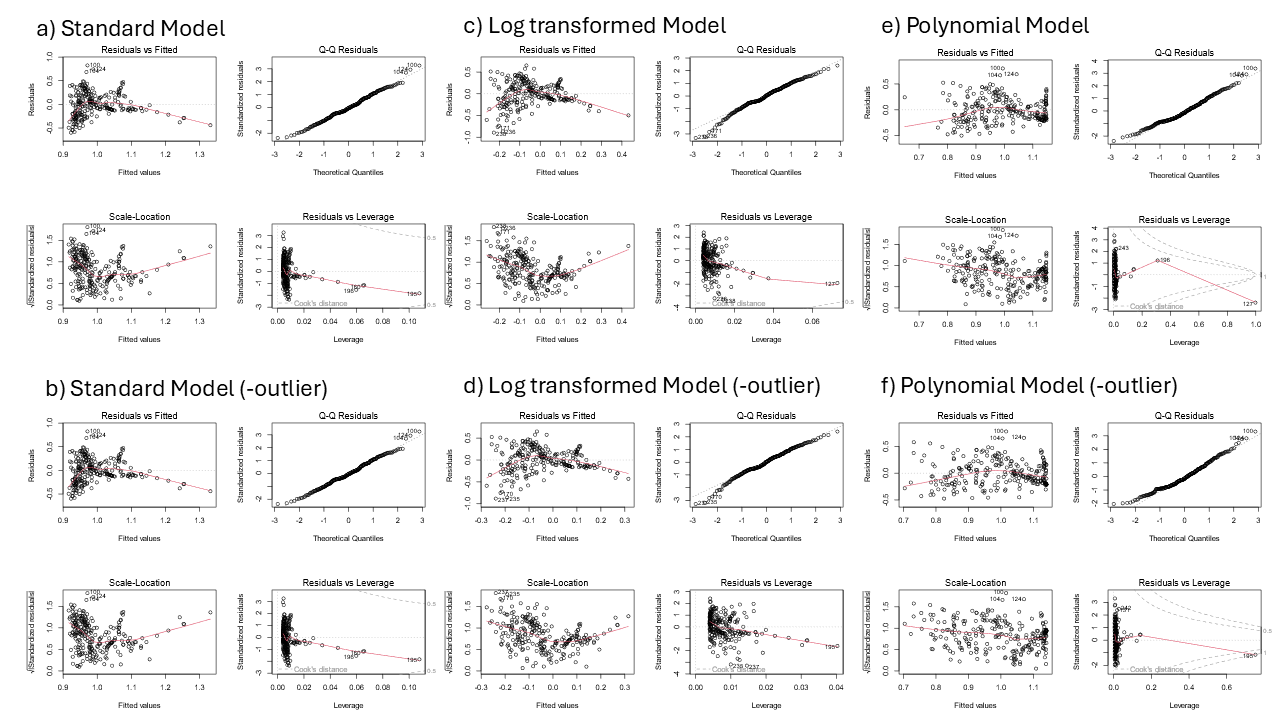
\includegraphics{Figures/Diagnostic plots.png}
\caption{Figure 4: diagnostic plots for all attempted models}
\end{figure}

It appears that the data violates the assumptions of a generalized
linear model under all attempted variations. For all models, both with
and without the outlier removed the `residuals vs fitted' and `scale vs
location' plots both show deviations from a flat horizontal
relationship, indicating that the data hetereoscedastic and the
relationship is non-linear.\\
The polynomial has the least violation of these assumptions, however the
outliers have a greater impact on the data, even when the most severe
outlier is removed.

\subsubsection{Spearman's rank correlation
coefficient}\label{spearmans-rank-correlation-coefficient}

Due to the data violating the assumptions of a linear model approach, we
decided to move forward with a non parametric approach using a
Spearman's rank correlation coefficient. Our data does match the
assumptions as it is monotonic with independent observations and as a
ranked method it is robust to outliers.

\begin{Shaded}
\begin{Highlighting}[]
\FunctionTok{cat}\NormalTok{(}\StringTok{"{-}{-}{-} Outcome of the Spearman\textquotesingle{}s rank correlation test {-}{-}{-}}\SpecialCharTok{\textbackslash{}n}\StringTok{"}\NormalTok{)}
\end{Highlighting}
\end{Shaded}

\begin{verbatim}
## --- Outcome of the Spearman's rank correlation test ---
\end{verbatim}

\begin{Shaded}
\begin{Highlighting}[]
\FunctionTok{cor.test}\NormalTok{(GTvL}\SpecialCharTok{$}\NormalTok{lambda, GTvL}\SpecialCharTok{$}\NormalTok{generation\_time, }\AttributeTok{method =} \StringTok{"spearman"}\NormalTok{)}
\end{Highlighting}
\end{Shaded}

\begin{verbatim}
## 
##  Spearman's rank correlation rho
## 
## data:  GTvL$lambda and GTvL$generation_time
## S = 1720894, p-value = 8.774e-09
## alternative hypothesis: true rho is not equal to 0
## sample estimates:
##       rho 
## 0.3547759
\end{verbatim}

The results of this test show that there is sufficient data to reject
our null hypotheses. There appears to be a relatively weak positive
relationship between the data. Considering the diagnostic plots from
earlier this relationship is likely non-linear.

\section{IUCN RedList}\label{iucn-redlist}

The International Union for the Conservation of Nature (IUCN) is a
collection of organisations that work together to aid in conservation
efforts ({``The IUCN Red List of Threatened Species,''} n.d.). the
RedList is a database containing many species and describing their
conservation status. Using this database, research and conservation
efforts can be effectively distributed between the species that most
need it.

\subsection{Acessing data (Q3)}\label{acessing-data-q3}

Due to issues with accessing the online database, instead we have
imported the data relevant to the comadre database from a csv (also
accessible on the github repository, under the folder ``Data'' (The
2025)).

\begin{Shaded}
\begin{Highlighting}[]
\DocumentationTok{\#\# loading the IUCNRedList data}
\NormalTok{IUCNData }\OtherTok{\textless{}{-}} \FunctionTok{read.csv}\NormalTok{(}\FunctionTok{here}\NormalTok{(}\StringTok{"Data"}\NormalTok{, }\StringTok{"IUCN\_comadre\_compadre.csv"}\NormalTok{))}
\CommentTok{\# combining with our comadre dataset}
\NormalTok{ComIUCN }\OtherTok{\textless{}{-}}\NormalTok{ ComSubFlag }\SpecialCharTok{\%\textgreater{}\%}
  \FunctionTok{left\_join}\NormalTok{(}\AttributeTok{x =}\NormalTok{ ., }\AttributeTok{y =}\NormalTok{ IUCNData, }\AttributeTok{by =} \StringTok{"SpeciesAccepted"}\NormalTok{) }\SpecialCharTok{\%\textgreater{}\%} 
  \FunctionTok{mutate}\NormalTok{(}\AttributeTok{IUCNstatus =} \FunctionTok{replace\_na}\NormalTok{(IUCNstatus, }\StringTok{"NE"}\NormalTok{))}
\CommentTok{\# producing a new column converting the two letter status codes into full words}
\NormalTok{ComIUCN }\OtherTok{\textless{}{-}}\NormalTok{ ComIUCN }\SpecialCharTok{\%\textgreater{}\%} 
  \FunctionTok{mutate}\NormalTok{(}\AttributeTok{IUCNstatLong =} \FunctionTok{case\_when}\NormalTok{(}
\NormalTok{    IUCNstatus }\SpecialCharTok{==} \StringTok{"EN"} \SpecialCharTok{\textasciitilde{}} \StringTok{"Endangered"}\NormalTok{,}
\NormalTok{    IUCNstatus }\SpecialCharTok{==} \StringTok{"VU"} \SpecialCharTok{\textasciitilde{}} \StringTok{"Vulnerable"}\NormalTok{,}
\NormalTok{    IUCNstatus }\SpecialCharTok{==} \StringTok{"NT"} \SpecialCharTok{\textasciitilde{}} \StringTok{"Near Threatened"}\NormalTok{,}
\NormalTok{    IUCNstatus }\SpecialCharTok{==} \StringTok{"LC"} \SpecialCharTok{\textasciitilde{}} \StringTok{"Least Concern"}\NormalTok{,}
\NormalTok{    IUCNstatus }\SpecialCharTok{==} \StringTok{"DD"} \SpecialCharTok{\textasciitilde{}} \StringTok{"Data Deficient"}\NormalTok{,}
\NormalTok{    IUCNstatus }\SpecialCharTok{==} \StringTok{"CR"} \SpecialCharTok{\textasciitilde{}} \StringTok{"Critically Endangered"}\NormalTok{,}
\NormalTok{    IUCNstatus }\SpecialCharTok{==} \StringTok{"EW"} \SpecialCharTok{\textasciitilde{}} \StringTok{"Extinct in the wild"}\NormalTok{,}
\NormalTok{    IUCNstatus }\SpecialCharTok{==} \StringTok{"EX"} \SpecialCharTok{\textasciitilde{}} \StringTok{"Extinct"}\NormalTok{,}
\NormalTok{    IUCNstatus }\SpecialCharTok{==} \StringTok{"NE"} \SpecialCharTok{\textasciitilde{}} \StringTok{"Not Evaluated"}\NormalTok{),}
    \AttributeTok{IUCNstatLong =} \FunctionTok{factor}\NormalTok{(IUCNstatLong, }
                        \AttributeTok{levels =} \FunctionTok{c}\NormalTok{(}\StringTok{"Extinct in the wild"}\NormalTok{,}
                                   \StringTok{"Extinct"}\NormalTok{,}\StringTok{"Endangered"}\NormalTok{,}
                                   \StringTok{"Vulnerable"}\NormalTok{,}
                                   \StringTok{"Near Threatened"}\NormalTok{,}
                                   \StringTok{"Least Concern"}\NormalTok{,}
                                   \StringTok{"Data Deficient"}\NormalTok{,}
                                   \StringTok{"Not Evaluated"}\NormalTok{)))}
\DocumentationTok{\#\# converting into a data frame}
\NormalTok{ComIUCN }\OtherTok{\textless{}{-}} \FunctionTok{as\_data\_frame}\NormalTok{(ComIUCN)}
\end{Highlighting}
\end{Shaded}

\subsection{analysis}\label{analysis}

\begin{Shaded}
\begin{Highlighting}[]
\NormalTok{IUCNVGTvL }\OtherTok{\textless{}{-}} \FunctionTok{subset}\NormalTok{(}\FunctionTok{as\_data\_frame}\NormalTok{(ComIUCN),generation\_time }\SpecialCharTok{\textless{}} \DecValTok{50}\NormalTok{) }\SpecialCharTok{\%\textgreater{}\%}
  \FunctionTok{select}\NormalTok{(lambda, generation\_time, IUCNstatLong) }\SpecialCharTok{\%\textgreater{}\%} 
  \FunctionTok{mutate}\NormalTok{(}\FunctionTok{across}\NormalTok{(}\FunctionTok{c}\NormalTok{(lambda, generation\_time), }
                \SpecialCharTok{\textasciitilde{}} \FunctionTok{na\_if}\NormalTok{(., }\ConstantTok{Inf}\NormalTok{))) }\SpecialCharTok{\%\textgreater{}\%} 
  \FunctionTok{mutate}\NormalTok{(}\FunctionTok{across}\NormalTok{(}\FunctionTok{c}\NormalTok{(lambda, generation\_time), }
                \SpecialCharTok{\textasciitilde{}} \FunctionTok{na\_if}\NormalTok{(., }\SpecialCharTok{{-}}\ConstantTok{Inf}\NormalTok{))) }\SpecialCharTok{\%\textgreater{}\%}
  \FunctionTok{drop\_na}\NormalTok{()}
\end{Highlighting}
\end{Shaded}

\textbf{generation time}

\begin{Shaded}
\begin{Highlighting}[]
\DocumentationTok{\#\# using a self made function to produce a boxplot comparing the varaibles}
\FunctionTok{boxplot}\NormalTok{(IUCNVGTvL, IUCNVGTvL}\SpecialCharTok{$}\NormalTok{IUCNstatLong, }\StringTok{"IUCN status"}\NormalTok{, IUCNVGTvL}\SpecialCharTok{$}\NormalTok{generation\_time, }\StringTok{"Generation Time (years)"}\NormalTok{, }\FunctionTok{paste}\NormalTok{(}\StringTok{"IUCN status vs generation time in the"}\NormalTok{, ClassName), }\StringTok{"IUCNvGT.svg"}\NormalTok{)}
\end{Highlighting}
\end{Shaded}

\begin{verbatim}
## pdf 
##   2
\end{verbatim}

\begin{Shaded}
\begin{Highlighting}[]
\DocumentationTok{\#\# running an ANOVA analysis}
\FunctionTok{cat}\NormalTok{(}\StringTok{"{-}{-}{-} ANOVA analysis of differences in generation time between conservation statuses {-}{-}{-}/n"}\NormalTok{)}
\end{Highlighting}
\end{Shaded}

\begin{verbatim}
## --- ANOVA analysis of differences in generation time between conservation statuses ---/n
\end{verbatim}

\begin{Shaded}
\begin{Highlighting}[]
\NormalTok{ANOVAGT }\OtherTok{\textless{}{-}} \FunctionTok{aov}\NormalTok{(generation\_time }\SpecialCharTok{\textasciitilde{}}\NormalTok{ IUCNstatLong, }\AttributeTok{data =}\NormalTok{ IUCNVGTvL)}
\FunctionTok{summary}\NormalTok{(ANOVAGT)}
\end{Highlighting}
\end{Shaded}

\begin{verbatim}
##               Df Sum Sq Mean Sq F value   Pr(>F)    
## IUCNstatLong   4    547  136.76   9.375 4.61e-07 ***
## Residuals    243   3545   14.59                     
## ---
## Signif. codes:  0 '***' 0.001 '**' 0.01 '*' 0.05 '.' 0.1 ' ' 1
\end{verbatim}

\begin{Shaded}
\begin{Highlighting}[]
\FunctionTok{cat}\NormalTok{(}\StringTok{"{-}{-}{-} Dunn\textquotesingle{}s test analysis of differences in generation time between conservation statuses {-}{-}{-}/n"}\NormalTok{)}
\end{Highlighting}
\end{Shaded}

\begin{verbatim}
## --- Dunn's test analysis of differences in generation time between conservation statuses ---/n
\end{verbatim}

\begin{Shaded}
\begin{Highlighting}[]
\FunctionTok{dunnTest}\NormalTok{(generation\_time }\SpecialCharTok{\textasciitilde{}}\NormalTok{ IUCNstatLong, }\AttributeTok{data =}\NormalTok{ IUCNVGTvL)}
\end{Highlighting}
\end{Shaded}

\begin{verbatim}
##                         Comparison          Z      P.unadj        P.adj
## 1       Endangered - Least Concern -1.0794234 2.803990e-01 8.411971e-01
## 2     Endangered - Near Threatened -2.2512459 2.436997e-02 1.462198e-01
## 3  Least Concern - Near Threatened -2.0339491 4.195672e-02 2.097836e-01
## 4       Endangered - Not Evaluated -1.4535475 1.460718e-01 5.842872e-01
## 5    Least Concern - Not Evaluated -0.8820864 3.777301e-01 7.554602e-01
## 6  Near Threatened - Not Evaluated  0.6528047 5.138822e-01 5.138822e-01
## 7          Endangered - Vulnerable -4.7704702 1.837964e-06 1.654168e-05
## 8       Least Concern - Vulnerable -5.2591784 1.447005e-07 1.447005e-06
## 9     Near Threatened - Vulnerable -3.0463839 2.316119e-03 1.621283e-02
## 10      Not Evaluated - Vulnerable -3.3630788 7.707835e-04 6.166268e-03
\end{verbatim}

\begin{figure}
\centering
\includesvg{Figures/IUCNvGT.svg}
\caption{Figure 5: Boxplot showing the generation time of species in
each conservation status category}
\end{figure}

There is a significant difference between vulnerable and the rest of the
categories, but none between the rest of the categories. This suggests
that species with longer generations are more likely to be categorised
as vulnerable. However, this relationship is not found with endangered
species, making the overall effect of generation time on vulnerability
confusing.

\textbf{Growth Rate}

\begin{Shaded}
\begin{Highlighting}[]
\DocumentationTok{\#\# using a self made function to produce a boxplot comparing the varaibles}
\FunctionTok{boxplot}\NormalTok{(IUCNVGTvL, IUCNVGTvL}\SpecialCharTok{$}\NormalTok{IUCNstatLong, }\StringTok{"IUCN status"}\NormalTok{, IUCNVGTvL}\SpecialCharTok{$}\NormalTok{lambda, }\StringTok{"Growth Rate (λ)"}\NormalTok{, }\FunctionTok{paste}\NormalTok{(}\StringTok{"IUCN status vs growth rate in the"}\NormalTok{, ClassName), }\StringTok{"IUCNvL.svg"}\NormalTok{ )}
\end{Highlighting}
\end{Shaded}

\begin{verbatim}
## pdf 
##   2
\end{verbatim}

\begin{Shaded}
\begin{Highlighting}[]
\DocumentationTok{\#\# running an ANOVA analysis}
\FunctionTok{cat}\NormalTok{(}\StringTok{"{-}{-}{-} ANOVA analysis of differences in growth rate between conservation statuses {-}{-}{-}/n"}\NormalTok{)}
\end{Highlighting}
\end{Shaded}

\begin{verbatim}
## --- ANOVA analysis of differences in growth rate between conservation statuses ---/n
\end{verbatim}

\begin{Shaded}
\begin{Highlighting}[]
\NormalTok{ANOVALambda }\OtherTok{\textless{}{-}} \FunctionTok{aov}\NormalTok{(lambda }\SpecialCharTok{\textasciitilde{}}\NormalTok{ IUCNstatLong, }\AttributeTok{data =}\NormalTok{ IUCNVGTvL)}
\FunctionTok{summary}\NormalTok{(ANOVALambda)}
\end{Highlighting}
\end{Shaded}

\begin{verbatim}
##               Df Sum Sq Mean Sq F value   Pr(>F)    
## IUCNstatLong   4  2.658  0.6644   11.29 2.03e-08 ***
## Residuals    243 14.299  0.0588                     
## ---
## Signif. codes:  0 '***' 0.001 '**' 0.01 '*' 0.05 '.' 0.1 ' ' 1
\end{verbatim}

\begin{Shaded}
\begin{Highlighting}[]
\FunctionTok{cat}\NormalTok{(}\StringTok{"{-}{-}{-} Dunn\textquotesingle{}s test analysis of differences in growth rate between conservation statuses {-}{-}{-}/n"}\NormalTok{)}
\end{Highlighting}
\end{Shaded}

\begin{verbatim}
## --- Dunn's test analysis of differences in growth rate between conservation statuses ---/n
\end{verbatim}

\begin{Shaded}
\begin{Highlighting}[]
\FunctionTok{dunnTest}\NormalTok{(lambda }\SpecialCharTok{\textasciitilde{}}\NormalTok{ IUCNstatLong, }\AttributeTok{data =}\NormalTok{ IUCNVGTvL)}
\end{Highlighting}
\end{Shaded}

\begin{verbatim}
##                         Comparison          Z      P.unadj        P.adj
## 1       Endangered - Least Concern -3.6302589 2.831371e-04 1.981960e-03
## 2     Endangered - Near Threatened -2.6289141 8.565800e-03 3.426320e-02
## 3  Least Concern - Near Threatened  0.4884560 6.252269e-01 6.252269e-01
## 4       Endangered - Not Evaluated -3.1939794 1.403261e-03 8.419568e-03
## 5    Least Concern - Not Evaluated -0.6799008 4.965673e-01 9.931346e-01
## 6  Near Threatened - Not Evaluated -0.8834502 3.769931e-01 1.000000e+00
## 7          Endangered - Vulnerable -6.1665962 6.977565e-10 6.977565e-09
## 8       Least Concern - Vulnerable -4.6878401 2.761037e-06 2.484933e-05
## 9     Near Threatened - Vulnerable -4.2084282 2.571532e-05 2.057226e-04
## 10      Not Evaluated - Vulnerable -3.0740389 2.111819e-03 1.055909e-02
\end{verbatim}

\begin{figure}
\centering
\includesvg{Figures/IUCNvL.svg}
\caption{Figure 6: Boxplot showing the population growth rate of species
in each conservation status category}
\end{figure}

In the case of population growth rate, Near threatened and least
concerned show no significant different from each other, or from species
which have not been evaluated. Endangered species show a significantly
decreased growth rate, as expected, whereas vulnerable species show an
increased growth rate. This is potentially due to implementation of
succsessful protective strategies increasing the growth rate of species
which are described as vulnerable.

\section{open tree of life (Q4)}\label{open-tree-of-life-q4}

The open tree of life is a collaborative effort to create a dynamic
phylogeny of the entire tree of life. It is openly accessible through an
API, but in this case it is being accessed through a .tre file of all of
the data relevant to the comadre dataset from the repository (Jones
2024) (also accessible on the github repository, under the folder
``Data'' (The 2025)).

\begin{Shaded}
\begin{Highlighting}[]
\DocumentationTok{\#\# Creating a new dataframe with each species only present once}
\NormalTok{ComSingle }\OtherTok{\textless{}{-}}\NormalTok{ ComIUCN[}\FunctionTok{which}\NormalTok{(}
  \FunctionTok{duplicated}\NormalTok{(ComIUCN}\SpecialCharTok{$}\NormalTok{SpeciesAccepted) }\SpecialCharTok{==} \ConstantTok{FALSE}\NormalTok{),]}

\DocumentationTok{\#\# wrangling data using the open tree of life online API}
\CommentTok{\# Creating a list of names from our dataframe that matches an entry in the open tree of life}
\NormalTok{ResNames }\OtherTok{\textless{}{-}}\NormalTok{ rotl}\SpecialCharTok{::}\FunctionTok{tnrs\_match\_names}\NormalTok{(}\AttributeTok{names =}\NormalTok{ ComSingle}\SpecialCharTok{$}\NormalTok{SpeciesAccepted)}
\CommentTok{\# adding the open tree of life id to our dataframe}
\NormalTok{ComSingle}\SpecialCharTok{$}\NormalTok{ott\_id }\OtherTok{\textless{}{-}}\NormalTok{ ResNames}\SpecialCharTok{$}\NormalTok{ott\_id}
\CommentTok{\# removing any values where there is no id}
\NormalTok{ComSingle }\OtherTok{\textless{}{-}}\NormalTok{ ComSingle[}\SpecialCharTok{{-}}\FunctionTok{which}\NormalTok{(}\FunctionTok{is.na}\NormalTok{(ComSingle}\SpecialCharTok{$}\NormalTok{ott\_id)),]}
\CommentTok{\# updating our list of mached names using only the ones with an id}
\NormalTok{ResNames }\OtherTok{\textless{}{-}}\NormalTok{ rotl}\SpecialCharTok{::}\FunctionTok{tnrs\_match\_names}\NormalTok{(}\AttributeTok{names =}\NormalTok{ ComSingle}\SpecialCharTok{$}\NormalTok{SpeciesAccepted)}
\CommentTok{\# putting this names into a new column in our dataframe}
\NormalTok{ComSingle}\SpecialCharTok{$}\NormalTok{OTL\_unique\_name }\OtherTok{\textless{}{-}}\NormalTok{ ResNames}\SpecialCharTok{$}\NormalTok{unique\_name}
\end{Highlighting}
\end{Shaded}

\begin{Shaded}
\begin{Highlighting}[]
\DocumentationTok{\#\# Loading in the tree data}
\NormalTok{Tree }\OtherTok{\textless{}{-}} \FunctionTok{read.tree}\NormalTok{(}\FunctionTok{here}\NormalTok{(}\StringTok{"Data"}\NormalTok{, }\StringTok{"COMPADRE{-}COMADRE\_Phylo\_June\_16\_2019.tre"}\NormalTok{))}

\DocumentationTok{\#\# remove NA and infinite values from our dataframe          }
\NormalTok{ComSingle }\OtherTok{\textless{}{-}}\NormalTok{ ComSingle  }\SpecialCharTok{\%\textgreater{}\%} 
  \FunctionTok{mutate}\NormalTok{(}\FunctionTok{across}\NormalTok{(}\FunctionTok{c}\NormalTok{(lambda, generation\_time), }\SpecialCharTok{\textasciitilde{}} \FunctionTok{na\_if}\NormalTok{(., }\ConstantTok{Inf}\NormalTok{))) }\SpecialCharTok{\%\textgreater{}\%} 
  \FunctionTok{mutate}\NormalTok{(}\FunctionTok{across}\NormalTok{(}\FunctionTok{c}\NormalTok{(lambda, generation\_time), }\SpecialCharTok{\textasciitilde{}} \FunctionTok{na\_if}\NormalTok{(., }\SpecialCharTok{{-}}\ConstantTok{Inf}\NormalTok{))) }\SpecialCharTok{\%\textgreater{}\%}
  \FunctionTok{drop\_na}\NormalTok{(lambda, generation\_time)}
                  
\DocumentationTok{\#\# Using the Open tree of life to create our own tree}
\CommentTok{\# Shortening the tip labels}
\NormalTok{Tree}\SpecialCharTok{$}\NormalTok{tip.label }\OtherTok{\textless{}{-}} \FunctionTok{gsub}\NormalTok{(}\StringTok{"\_"}\NormalTok{, }\StringTok{" "}\NormalTok{, Tree}\SpecialCharTok{$}\NormalTok{tip.label)}
\CommentTok{\# Removing species which aren\textquotesingle{}t in our dataframe}
\NormalTok{PrunedTree }\OtherTok{\textless{}{-}} \FunctionTok{drop.tip}\NormalTok{(Tree, }\FunctionTok{setdiff}\NormalTok{(Tree}\SpecialCharTok{$}\NormalTok{tip.label, ComSingle}\SpecialCharTok{$}\NormalTok{OTL\_unique\_name))}
\CommentTok{\# alterning the order of our dataframe to map the tree}
\NormalTok{ComSingle }\OtherTok{\textless{}{-}}\NormalTok{ ComSingle[}\FunctionTok{match}\NormalTok{(PrunedTree}\SpecialCharTok{$}\NormalTok{tip.label,ComSingle}\SpecialCharTok{$}\NormalTok{OTL\_unique\_name),]}
\CommentTok{\# setting the species names as the row names}
\FunctionTok{row.names}\NormalTok{(ComSingle) }\OtherTok{\textless{}{-}}\NormalTok{ ComSingle}\SpecialCharTok{$}\NormalTok{OTL\_unique\_name}

\DocumentationTok{\#\# Plotting our Pruned tree}
\FunctionTok{svglite}\NormalTok{(}\FunctionTok{here}\NormalTok{(}\StringTok{"Figures"}\NormalTok{, }\StringTok{"PrunedTree.svg"}\NormalTok{), }\AttributeTok{width =} \DecValTok{8}\NormalTok{, }\AttributeTok{height =} \DecValTok{8}\NormalTok{, }\AttributeTok{scaling =} \FloatTok{0.9}\NormalTok{) }
\FunctionTok{plot}\NormalTok{(PrunedTree, }\AttributeTok{fsize =} \FunctionTok{c}\NormalTok{(}\FloatTok{0.7}\NormalTok{,}\FloatTok{0.8}\NormalTok{)) }
\FunctionTok{dev.off}\NormalTok{()}
\end{Highlighting}
\end{Shaded}

\begin{verbatim}
## pdf 
##   2
\end{verbatim}

\includesvg{Figures/PrunedTree.svg}

\subsection{Plotting phylogeny with population
parameters}\label{plotting-phylogeny-with-population-parameters}

\subsubsection{\texorpdfstring{\textbf{growth
rate}}{growth rate}}\label{growth-rate}

\begin{Shaded}
\begin{Highlighting}[]
\DocumentationTok{\#\# Creating a list containing the Log of the growth rate attached to the species name}
\NormalTok{LogL }\OtherTok{\textless{}{-}} \FunctionTok{log}\NormalTok{(}\FunctionTok{setNames}\NormalTok{(ComSingle}\SpecialCharTok{$}\NormalTok{lambda, }\FunctionTok{row.names}\NormalTok{(ComSingle)))}

\DocumentationTok{\#\# creating a phylogenetic tree coloured based on the population growth rate}
\NormalTok{ContMapL }\OtherTok{\textless{}{-}} \FunctionTok{contMap}\NormalTok{(PrunedTree, LogL,}\AttributeTok{plot=}\ConstantTok{FALSE}\NormalTok{,}\AttributeTok{res=}\DecValTok{1000}\NormalTok{,}
                    \AttributeTok{method=}\StringTok{"anc.ML"}\NormalTok{) }
\NormalTok{ContMapL }\OtherTok{\textless{}{-}} \FunctionTok{setMap}\NormalTok{(ContMapL, }\FunctionTok{c}\NormalTok{(}\StringTok{"white"}\NormalTok{,}\StringTok{"\#FFFFB2"}\NormalTok{,}\StringTok{"\#FECC5C"}\NormalTok{,}
                               \StringTok{"\#FD8D3C"}\NormalTok{,}\StringTok{"\#E31A1C"}\NormalTok{))}

\DocumentationTok{\#\# Plotting the phylogenetic tree}
\FunctionTok{svglite}\NormalTok{(}\FunctionTok{here}\NormalTok{(}\StringTok{"Figures"}\NormalTok{, }\StringTok{"ContMapLambda.svg"}\NormalTok{), }\AttributeTok{width =} \DecValTok{8}\NormalTok{, }\AttributeTok{height =} \DecValTok{8}\NormalTok{, }\AttributeTok{scaling =} \FloatTok{1.2}\NormalTok{) }
\FunctionTok{plot}\NormalTok{(ContMapL, }\AttributeTok{fsize =} \FunctionTok{c}\NormalTok{(}\FloatTok{0.7}\NormalTok{,}\FloatTok{0.8}\NormalTok{), }\AttributeTok{leg.txt =} 
       \StringTok{"log(population growth rate)"}\NormalTok{) }
\FunctionTok{dev.off}\NormalTok{()}
\end{Highlighting}
\end{Shaded}

\begin{verbatim}
## pdf 
##   2
\end{verbatim}

\includesvg{Figures/ContMapLambda.svg}

It doesn't appear that the population growth rate does is not affected
by phylogenetic inertia. There is no clear clustering or relation
between individuals with either particularly high or low growth rates,
with growth rates often being very different from closely related
individuals.

\subsubsection{\texorpdfstring{\textbf{Generation
time}}{Generation time}}\label{generation-time}

\begin{Shaded}
\begin{Highlighting}[]
\DocumentationTok{\#\# Creating a list containing the Log of the generation time attached to the species name}
\NormalTok{LogGT }\OtherTok{\textless{}{-}} \FunctionTok{log}\NormalTok{(}\FunctionTok{setNames}\NormalTok{(ComSingle}\SpecialCharTok{$}\NormalTok{generation\_time, }\FunctionTok{row.names}\NormalTok{(ComSingle)))}

\DocumentationTok{\#\# creating a phylogenetic tree coloured based on the generation time}
\NormalTok{ContMapGT }\OtherTok{\textless{}{-}} \FunctionTok{contMap}\NormalTok{(PrunedTree, LogGT,}\AttributeTok{plot=}\ConstantTok{FALSE}\NormalTok{,}\AttributeTok{res=}\DecValTok{200}\NormalTok{, }
                     \AttributeTok{method=}\StringTok{"anc.ML"}\NormalTok{)}
\NormalTok{ContMapGT }\OtherTok{\textless{}{-}} \FunctionTok{setMap}\NormalTok{(ContMapGT, }\FunctionTok{c}\NormalTok{(}\StringTok{"white"}\NormalTok{,}\StringTok{"light blue"}\NormalTok{,}\StringTok{"blue"}\NormalTok{,}
                                 \StringTok{"violet"}\NormalTok{,}\StringTok{"purple"}\NormalTok{))}

\DocumentationTok{\#\# Plotting the phylogenetic tree}
\FunctionTok{svglite}\NormalTok{(}\FunctionTok{here}\NormalTok{(}\StringTok{"Figures"}\NormalTok{, }\StringTok{"ContMapGT.svg"}\NormalTok{), }
        \AttributeTok{width =} \DecValTok{8}\NormalTok{, }\AttributeTok{height =} \DecValTok{8}\NormalTok{, }\AttributeTok{scaling =} \FloatTok{1.2}\NormalTok{)}
\FunctionTok{plot}\NormalTok{(ContMapGT, }\AttributeTok{fsize=}\FunctionTok{c}\NormalTok{(}\FloatTok{0.7}\NormalTok{,}\FloatTok{0.8}\NormalTok{), }\AttributeTok{leg.txt =} 
       \StringTok{"log(generation time) (years)"}\NormalTok{)}
\FunctionTok{dev.off}\NormalTok{()}
\end{Highlighting}
\end{Shaded}

\begin{verbatim}
## pdf 
##   2
\end{verbatim}

\includesvg{Figures/ContMapGT.svg}

Generation time on the other hand shows a substantial effect of
phylogenetic inertia. It is generally more closely matched between
closely related individuals than those which are distantly related and
shows strong clustering.

\subsection{population performance
(Q5)}\label{population-performance-q5}

This final phylogeny shows Whether each species is increasing
(population growth rate \textgreater{} 1) or decreasing (population
growth rate \textless1) as well as their conservation status.

using code from ({``Exercise 15: Plotting Methods for Phylogenies \&
Comparative Data in r,''} n.d.)

\begin{Shaded}
\begin{Highlighting}[]
\DocumentationTok{\#\# Creating a list of either "Increase" if growth rate is greater than one, or "Decrease" if it is less}
\NormalTok{PopPerf }\OtherTok{\textless{}{-}} \FunctionTok{as\_data\_frame}\NormalTok{(ComSingle}\SpecialCharTok{$}\NormalTok{lambda) }\SpecialCharTok{\%\textgreater{}\%} 
  \FunctionTok{mutate}\NormalTok{(}\AttributeTok{category =} \FunctionTok{factor}\NormalTok{(}
    \FunctionTok{case\_when}\NormalTok{(value }\SpecialCharTok{\textless{}} \DecValTok{1}  \SpecialCharTok{\textasciitilde{}} \StringTok{"Decrease"}\NormalTok{,}
\NormalTok{              value }\SpecialCharTok{\textgreater{}} \DecValTok{1}  \SpecialCharTok{\textasciitilde{}} \StringTok{"Increase"}\NormalTok{)))}

\DocumentationTok{\#\# adding the conservation status to the tip labels}
\CommentTok{\# seperating creating a new column in our dataframe combining the status and the species name into one string}
\NormalTok{ComSingle}\SpecialCharTok{$}\NormalTok{TipName }\OtherTok{\textless{}{-}} \FunctionTok{paste}\NormalTok{(ComSingle}\SpecialCharTok{$}\NormalTok{IUCNstatus,}
\NormalTok{                           ComSingle}\SpecialCharTok{$}\NormalTok{OTL\_unique\_name, }
                           \AttributeTok{sep =} \StringTok{" "}\NormalTok{)}
\CommentTok{\# replacing the tip labels with these new strings}
\NormalTok{PrunedTree}\SpecialCharTok{$}\NormalTok{tip.label }\OtherTok{\textless{}{-}}\NormalTok{ ComSingle}\SpecialCharTok{$}\NormalTok{TipName}
\CommentTok{\# replacing PopPerf with a list of factors as named by our new tip labels}
\NormalTok{PopPerf }\OtherTok{\textless{}{-}} \FunctionTok{as.factor}\NormalTok{(}\FunctionTok{setNames}\NormalTok{(PopPerf}\SpecialCharTok{$}\NormalTok{category,}
\NormalTok{            ComSingle}\SpecialCharTok{$}\NormalTok{TipName))}

\DocumentationTok{\#\# plotting our new tree}
\FunctionTok{svglite}\NormalTok{(}\FunctionTok{here}\NormalTok{(}\StringTok{"Figures"}\NormalTok{, }\StringTok{"PerfTree.svg"}\NormalTok{), }\AttributeTok{width =} \DecValTok{8}\NormalTok{,}
          \AttributeTok{height =} \DecValTok{8}\NormalTok{,}
          \AttributeTok{scaling =} \FloatTok{0.9}\NormalTok{)}
\CommentTok{\# plotting a tree with dots coloured depending on whether the growth rate is greater than or less than 1}
\FunctionTok{dotTree}\NormalTok{(PrunedTree, PopPerf, }\AttributeTok{colors =} \FunctionTok{setNames}\NormalTok{(}
                     \FunctionTok{c}\NormalTok{(}\StringTok{"\#EA0000"}\NormalTok{, }\StringTok{"\#1E88E5"}\NormalTok{),}
                     \FunctionTok{c}\NormalTok{(}\StringTok{"Decrease"}\NormalTok{,}\StringTok{"Increase"}\NormalTok{)),}
        \AttributeTok{ftype=}\StringTok{"i"}\NormalTok{, )}
\FunctionTok{dev.off}\NormalTok{()}
\end{Highlighting}
\end{Shaded}

\begin{verbatim}
## pdf 
##   2
\end{verbatim}

\includesvg{Figures/PerfTree.svg}

\begin{center}\rule{0.5\linewidth}{0.5pt}\end{center}

\section{Appendix}\label{appendix}

\subsection{references}\label{references}

\phantomsection\label{refs}
\begin{CSLReferences}{1}{0}
\bibitem[\citeproctext]{ref-exercise}
{``Exercise 15: Plotting Methods for Phylogenies \& Comparative Data in
r.''} n.d.
\url{http://www.phytools.org/Cordoba2017/ex/15/Plotting-methods.html}.

\bibitem[\citeproctext]{ref-jones2024}
Jones, Owen. 2024. \emph{Jonesor/compadreDB}.
\url{https://github.com/jonesor/compadreDB}.

\bibitem[\citeproctext]{ref-nichols}
Nichols, David. n.d. {``Coloring for Colorblindness.''}
\url{http://www.davidmathlogic.com/colorblind/}.

\bibitem[\citeproctext]{ref-salguero-guxf3mez2016}
Salguero-Gómez, Roberto, Owen R. Jones, C. Ruth Archer, Christoph Bein,
Hendrik De Buhr, Claudia Farack, Fränce Gottschalk, et al. 2016.
{``COMADRE : A Global Data Base of Animal Demography.''} Edited by Tim
Coulson. \emph{Journal of Animal Ecology} 85 (2): 371--84.
\url{https://doi.org/10.1111/1365-2656.12482}.

\bibitem[\citeproctext]{ref-theiucn}
{``The IUCN Red List of Threatened Species.''} n.d.
\url{https://www.iucnredlist.org/en}.

\bibitem[\citeproctext]{ref-the2025}
The, Nedstar. 2025. {``The-Nedstar/LargeDatasets.''}
\url{https://github.com/The-Nedstar/LargeDatasets}.

\bibitem[\citeproctext]{ref-whitlock2020analysis}
Whitlock, Michael C., and Dolph Schluter. 2020. \emph{The Analysis of
Biological Data}. 3rd ed. New York: Macmillan Learning.

\end{CSLReferences}

\subsection{Contents of the Functions.R
file}\label{contents-of-the-functions.r-file}

Can also be found on the anonymised github repository (The 2025).

\begin{Shaded}
\begin{Highlighting}[]
\DocumentationTok{\#\#\#\#\#\#\#\#\#\#\#\#\#\#\#\#\#\#\#\#\#\#\#\#\#\#\#\#\#\#\#\#\#\#\#\#\#\#\#\#\#\#\#}
\CommentTok{\# Functions for the Large Dataset assignment}
\CommentTok{\# author: anonymous}
\DocumentationTok{\#\#\#\#\#\#\#\#\#\#\#\#\#\#\#\#\#\#\#\#\#\#\#\#\#\#\#\#\#\#\#\#\#\#\#\#\#\#\#\#\#\#\#}

\DocumentationTok{\#\#\# creation of a histogram}
\NormalTok{histogram }\OtherTok{\textless{}{-}} \ControlFlowTok{function}\NormalTok{(Data, Xaxis, Xtitle, Title, BW, Line, File)\{}
  \DocumentationTok{\#\# defining the histogram}
\NormalTok{  temp }\OtherTok{\textless{}{-}} \FunctionTok{ggplot}\NormalTok{(Data, }\FunctionTok{aes}\NormalTok{(}\AttributeTok{x =}\NormalTok{ Xaxis)) }\SpecialCharTok{+}
    \FunctionTok{geom\_histogram}\NormalTok{(}\FunctionTok{aes}\NormalTok{(}\AttributeTok{fill =} \FunctionTok{as.factor}\NormalTok{(}\FunctionTok{floor}\NormalTok{(..x.. }\SpecialCharTok{/}\NormalTok{ BW) }\SpecialCharTok{\%\%} \DecValTok{2}\NormalTok{)), }\CommentTok{\# alternative colours}
                   \AttributeTok{binwidth =}\NormalTok{ BW, }\AttributeTok{boundary =} \DecValTok{1}\NormalTok{, }\CommentTok{\# ensuring it is split at the value 1}
                   \AttributeTok{colour =} \StringTok{"black"}\NormalTok{, }\AttributeTok{size =} \FloatTok{0.4}\NormalTok{) }\SpecialCharTok{+}
\NormalTok{    (}\ControlFlowTok{if}\NormalTok{ (Line }\SpecialCharTok{==} \ConstantTok{TRUE}\NormalTok{) \{ }\CommentTok{\# only carrying out if specified}
      \FunctionTok{geom\_vline}\NormalTok{(}\AttributeTok{xintercept =} \DecValTok{1}\NormalTok{, }\AttributeTok{colour =} \StringTok{"red"}\NormalTok{, }
                 \AttributeTok{size =} \FloatTok{1.3}\NormalTok{, }\AttributeTok{linetype =} \StringTok{"21"}\NormalTok{)\}) }\SpecialCharTok{+} \CommentTok{\# creates a vertical line at the value 1}
    \FunctionTok{scale\_fill\_manual}\NormalTok{(}\AttributeTok{values =} \FunctionTok{c}\NormalTok{(}\StringTok{"\#707070"}\NormalTok{, }\StringTok{"\#555555"}\NormalTok{)) }\SpecialCharTok{+} \CommentTok{\# specifying alternating colours}
    \FunctionTok{theme\_bw}\NormalTok{()}\SpecialCharTok{+}
    \FunctionTok{theme}\NormalTok{(}
      \AttributeTok{legend.position =} \StringTok{"none"}\NormalTok{, }\CommentTok{\# removing the legend}
      \AttributeTok{axis.title =} \FunctionTok{element\_text}\NormalTok{(}\AttributeTok{size =} \DecValTok{14}\NormalTok{),}
      \AttributeTok{title =} \FunctionTok{element\_text}\NormalTok{(}\AttributeTok{size =} \DecValTok{14}\NormalTok{)}
\NormalTok{    ) }\SpecialCharTok{+}
    \FunctionTok{xlab}\NormalTok{(Xtitle) }\SpecialCharTok{+}
    \FunctionTok{ylab}\NormalTok{(}\StringTok{"Frequency"}\NormalTok{) }\SpecialCharTok{+}
    \FunctionTok{ggtitle}\NormalTok{(Title)}
  \DocumentationTok{\#\# saving the graph as a .svg}
  \FunctionTok{svglite}\NormalTok{(}\FunctionTok{here}\NormalTok{(}\StringTok{"Figures"}\NormalTok{, File), }\AttributeTok{width =} \DecValTok{10}\NormalTok{,}
          \AttributeTok{height =} \DecValTok{6}\NormalTok{,}
          \AttributeTok{scaling =} \FloatTok{1.1}\NormalTok{)}
  \FunctionTok{print}\NormalTok{(temp)}
  \FunctionTok{dev.off}\NormalTok{()}
\NormalTok{\}}

\DocumentationTok{\#\#\# create a scatterplot}
\NormalTok{scatterplot }\OtherTok{\textless{}{-}} \ControlFlowTok{function}\NormalTok{(Data, Xaxis, Xtitle, Yaxis, Ytitle, Title, Line, File)\{}
  \DocumentationTok{\#\# creating the scatterplot}
\NormalTok{  temp }\OtherTok{\textless{}{-}} \FunctionTok{ggplot}\NormalTok{(Data, }\FunctionTok{aes}\NormalTok{(}\AttributeTok{x =}\NormalTok{ Xaxis, }\AttributeTok{y =}\NormalTok{ Yaxis)) }\SpecialCharTok{+}
    \FunctionTok{geom\_point}\NormalTok{(}\AttributeTok{colour =} \StringTok{"darkblue"}\NormalTok{)}\SpecialCharTok{+}
\NormalTok{    (}\ControlFlowTok{if}\NormalTok{ (Line }\SpecialCharTok{==} \ConstantTok{TRUE}\NormalTok{) \{ }\CommentTok{\# Only running if specified}
      \FunctionTok{geom\_smooth}\NormalTok{(}\AttributeTok{method =} \StringTok{"lm"}\NormalTok{, }\AttributeTok{se =} \ConstantTok{TRUE}\NormalTok{, }\AttributeTok{linetype =} \StringTok{"solid"}\NormalTok{, }
                  \AttributeTok{colour =} \StringTok{"darkred"}\NormalTok{)\}) }\SpecialCharTok{+} \CommentTok{\# creating a line defined by a generalised linear model}
    \FunctionTok{theme\_bw}\NormalTok{()}\SpecialCharTok{+}
    \FunctionTok{theme}\NormalTok{(}
      \AttributeTok{legend.position =} \StringTok{"none"}\NormalTok{, }\CommentTok{\# removing the legend}
      \AttributeTok{axis.title =} \FunctionTok{element\_text}\NormalTok{(}\AttributeTok{size =} \DecValTok{14}\NormalTok{),}
      \AttributeTok{title =} \FunctionTok{element\_text}\NormalTok{(}\AttributeTok{size =} \DecValTok{14}\NormalTok{)}
\NormalTok{    ) }\SpecialCharTok{+}
    \FunctionTok{xlab}\NormalTok{(Xtitle) }\SpecialCharTok{+}
    \FunctionTok{ylab}\NormalTok{(Ytitle) }\SpecialCharTok{+}
    \FunctionTok{ggtitle}\NormalTok{(Title)}
  \DocumentationTok{\#\# saving as a .svg}
  \FunctionTok{svglite}\NormalTok{(}\FunctionTok{here}\NormalTok{(}\StringTok{"Figures"}\NormalTok{, File), }\AttributeTok{width =} \DecValTok{10}\NormalTok{,}
          \AttributeTok{height =} \DecValTok{6}\NormalTok{,}
          \AttributeTok{scaling =} \FloatTok{1.1}\NormalTok{)}
  \FunctionTok{print}\NormalTok{(temp)}
  \FunctionTok{dev.off}\NormalTok{()}
\NormalTok{\}}

\DocumentationTok{\#\#\# Create Diagnostic plots}
\NormalTok{diagnostic\_plots }\OtherTok{\textless{}{-}} \ControlFlowTok{function}\NormalTok{(File, Model) \{}
  \DocumentationTok{\#\# saving plot as an SVG}
  \FunctionTok{svglite}\NormalTok{(}\FunctionTok{here}\NormalTok{(}\StringTok{"Figures"}\NormalTok{, File), }\AttributeTok{width =} \DecValTok{10}\NormalTok{,}
          \AttributeTok{height =} \DecValTok{8}\NormalTok{,}
          \AttributeTok{scaling =} \FloatTok{1.3}\NormalTok{)}
  \DocumentationTok{\#\# creating a multi plot}
  \CommentTok{\# defining multi plot layout}
  \FunctionTok{par}\NormalTok{(}\AttributeTok{mfrow=}\FunctionTok{c}\NormalTok{(}\DecValTok{2}\NormalTok{,}\DecValTok{2}\NormalTok{))}
  \CommentTok{\# combining each diagnostic plot into one multi plot}
\NormalTok{  DiaPlots }\OtherTok{\textless{}{-}}\NormalTok{ (}\FunctionTok{plot}\NormalTok{(Model,}\DecValTok{1}\NormalTok{) }\SpecialCharTok{|} \FunctionTok{plot}\NormalTok{(Model,}\DecValTok{2}\NormalTok{)) }\SpecialCharTok{/}\NormalTok{ (}\FunctionTok{plot}\NormalTok{(Model,}\DecValTok{3}\NormalTok{) }\SpecialCharTok{|} \FunctionTok{plot}\NormalTok{(Model,}\DecValTok{5}\NormalTok{))}
  \FunctionTok{dev.off}\NormalTok{()}
\NormalTok{\}}

\DocumentationTok{\#\#\# create a boxplot}
\NormalTok{boxplot }\OtherTok{\textless{}{-}} \ControlFlowTok{function}\NormalTok{(Data, Xaxis, Xtitle, Yaxis, Ytitle, Title, File)\{}
  \DocumentationTok{\#\# defining the boxplot}
\NormalTok{  temp }\OtherTok{\textless{}{-}} \FunctionTok{ggplot}\NormalTok{(Data, }\FunctionTok{aes}\NormalTok{(}\AttributeTok{x =}\NormalTok{ Xaxis, }\AttributeTok{y =}\NormalTok{ Yaxis, }\AttributeTok{fill =}\NormalTok{ Xaxis)) }\SpecialCharTok{+}
    \FunctionTok{geom\_boxplot}\NormalTok{() }\SpecialCharTok{+}
    \FunctionTok{geom\_beeswarm}\NormalTok{(}\AttributeTok{alpha =} \FloatTok{0.6}\NormalTok{, }\AttributeTok{size =} \FloatTok{0.75}\NormalTok{, }\AttributeTok{corral.width =} \FloatTok{0.5}\NormalTok{) }\SpecialCharTok{+}
    \FunctionTok{scale\_fill\_manual}\NormalTok{(}\AttributeTok{values =} \FunctionTok{c}\NormalTok{(}\StringTok{"\#E89494"}\NormalTok{, }\StringTok{"\#A4DFE4"}\NormalTok{, }\StringTok{"\#8082E4"}\NormalTok{,}
                                 \StringTok{"\#F2D16F"}\NormalTok{, }\StringTok{"\#EC89E4"}\NormalTok{)) }\SpecialCharTok{+} \CommentTok{\# defining colours}
    \FunctionTok{theme\_bw}\NormalTok{() }\SpecialCharTok{+}
    \FunctionTok{theme}\NormalTok{(}
      \AttributeTok{legend.position =} \StringTok{"none"}\NormalTok{, }\CommentTok{\# removing the legend}
      \AttributeTok{axis.title =} \FunctionTok{element\_text}\NormalTok{(}\AttributeTok{size =} \DecValTok{14}\NormalTok{),}
      \AttributeTok{title =} \FunctionTok{element\_text}\NormalTok{(}\AttributeTok{size =} \DecValTok{14}\NormalTok{)}
\NormalTok{    ) }\SpecialCharTok{+}
    \FunctionTok{xlab}\NormalTok{(Xtitle) }\SpecialCharTok{+}
    \FunctionTok{ylab}\NormalTok{(Ytitle) }\SpecialCharTok{+}
    \FunctionTok{ggtitle}\NormalTok{(Title)}
  \DocumentationTok{\#\# saving as a .svg}
  \FunctionTok{svglite}\NormalTok{(}\FunctionTok{here}\NormalTok{(}\StringTok{"Figures"}\NormalTok{, File), }\AttributeTok{width =} \DecValTok{10}\NormalTok{,}
          \AttributeTok{height =} \DecValTok{6}\NormalTok{,}
          \AttributeTok{scaling =} \FloatTok{1.3}\NormalTok{)}
  \FunctionTok{print}\NormalTok{(temp)}
  \FunctionTok{dev.off}\NormalTok{()}
\NormalTok{\}}
\end{Highlighting}
\end{Shaded}


\end{document}
